\chapter{Conclusions \& Recommendations}
Creating an Alexa for the first time was intimidating. Learning how to set up the skill was the hardest part as it was completely new to us. Learning how the Alexa skill is all wired up was a big challenge, but as time went on we figured out slowly how to get each component 'talking' with one another. Once we had each component working we rapidly were able to get the application together using Node.js. The application was hard to setup as it was out first time but easy to develop for once setup.

One of the big features of Alexa is the huge market of users it has, increasing the reach of the application. The application is hosted on \hyperlink{https://www.amazon.co.uk/Cian-GameFinder/dp/B07QH4N2GG}{Amazon UK} using the Alexa Developer Console to setup the store page. Setting up the store page worked in a very similar way to how Microsoft's Windows store works. There is a two stage verification of the application. An automatic review and a manual review. The automatic review does a basic test on the intents setup, checks if the five basic intents are setup and if the skill has the information for the store page setup. The manual review can only be done when the previous automatic review has passed. The manual review is done by an Amazon Echo employee who is given instructions by the developer on how to run the skill. The tester then tests the skill and gives feedback on how well it runs and if any changes are needed.

\begin{figure}[h!]
  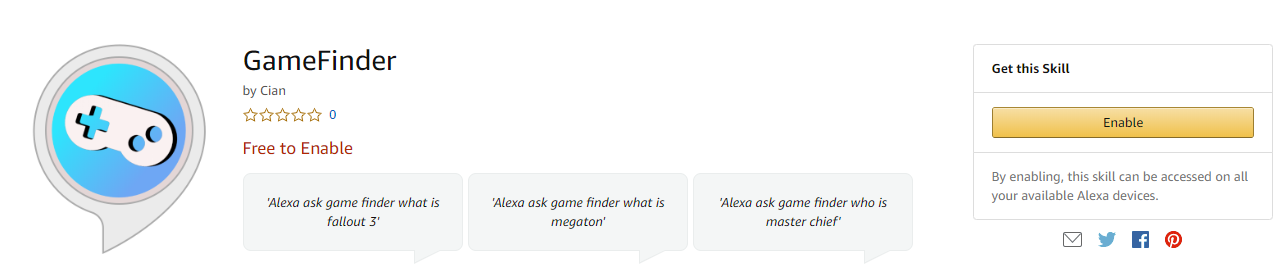
\includegraphics[width=\linewidth]{Store.PNG}
  \caption{Amazon Store}
  \label{fig:amazonstore}
\end{figure}

Once the tests were passed within a few hours the skill was live on the \hyperlink{https://www.amazon.co.uk/Cian-GameFinder/dp/B07QH4N2GG}{Amazon UK} store for free.

\begin{figure}[h!]
  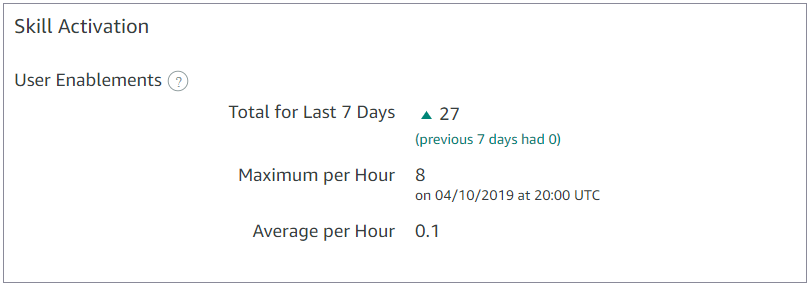
\includegraphics[width=\linewidth]{Skill.PNG}
  \caption{Amazon Store}
  \label{fig:amazonstore}
\end{figure}

Within two days we had 27 total users and 8 requests made in a single hour. We have gotten no bug reports and the AWS Lambda logs show no errors with the requests users have made.

Voice assistants have had huge growth in the last few years thank in part due to devices like the Echo and voice assistant on our phones such as Siri for IPhone and Cortana for Microsoft. Voice assistants are rapidly become a bigger part of our lives and creating an application to to get a greater understanding on how they work was very worth while.

Overall the experience in developing an Alexa skill was great. It was a completely new experience to us and we did learn a great deal more about how voice controlled assistants operate and interpret what the user say. I would recommend others to develop a gesture application using the Alexa skill framework. It's very flexible and give developers a huge market of users to get feedback from.
